\documentclass[../ai_in_finance]{subfiles}
\usepackage[margin=1in]{geometry}
\usepackage{tikz}
\usetikzlibrary{positioning}
\usepackage{amsmath}
\usepackage{amssymb}
\usepackage{booktabs}
\usepackage{floatrow}
\usepackage{draftwatermark}

\SetWatermarkText{Wulin.Suo@Queensu.ca}
\SetWatermarkScale{1.4}
\SetWatermarkColor{gray!35}
\SetWatermarkAngle{90}
\SetWatermarkHorCenter{0.94\paperwidth}
\SetWatermarkVerCenter{0.5\paperheight}

\usepackage{makeidx}
\makeindex

\begin{document}

\chapter{Fraud Detection, Compliance, and Financial Crime}

\section{Introduction}

Chapter 1 previewed this chapter with a single number: a fraud detection model that correctly flags 95\% of actual fraud and mistakenly flags only 3\% of legitimate transactions still produces a flagged transaction that is fraudulent only about 24\% of the time, because fraud is rare enough that even a small false-positive rate generates many more false alarms than true detections. That number is not a curiosity; it is the central operating constraint of every fraud detection and anti-money-laundering (AML) system in the financial industry, and this chapter is built around understanding and managing it. Chapter 6 developed classification models and the confusion matrix\index{confusion matrix} in the abstract, using loan default as the running example; Chapter 9 applied a closely related toolkit, logistic regression\index{logistic regression}, scoring, and rating models, to credit risk. This chapter applies the same statistical machinery to a different, related family of problems: detecting fraud, laundered money, and other financial crime, where the base rate of the event being detected is typically far lower than a loan portfolio's default rate, and where the operational and legal consequences of a false positive or a missed detection are correspondingly distinct.

Four worked examples run through the chapter. The Bayes' theorem\index{Bayes' theorem} calculation from Chapter 1 is scaled up to a full day of transaction volume, converting an abstract posterior probability into a concrete daily confusion matrix and an alert queue a compliance team actually has to work through. A small fraud-scoring logistic regression, in the same spirit as Chapter 6's confusion matrix example and Chapter 9's credit-scoring model, illustrates how a handful of transaction features combine into a fraud probability, and where such a model can still miss a genuine case. A Kaplan-Meier\index{Kaplan-Meier estimator} survival analysis, a technique new to this book, estimates how long flagged accounts typically remain active before a confirmed fraud closes them, introducing censored observations, data this book has not previously had to handle. Finally, a structuring example shows how AML monitoring rules are built around a specific, legally defined reporting threshold, and how criminals attempt to evade it.

\section{Detecting Fraud}

Fraud is a rare-event classification problem, and this part builds a detector while confronting exactly how rare the positives are.

\subsection{The Landscape of Financial Crime and Where AI Fits}
\label{sec:crime-taxonomy}

Suppose a bank builds an excellent fraud-scoring model, one that catches nearly every stolen-card transaction, and considers its detection obligations largely satisfied, only to later face a regulatory fine for failing to flag an unrelated money-laundering scheme that a fraud model was never designed to catch in the first place. ``Fraud detection'' understates the breadth of what financial institutions are legally required to monitor for.

Table~\ref{tab:crime_taxonomy} organizes the main categories of financial crime this book touches on, the detection approach each typically relies on, and where it is developed.

\begin{table}[htbp]
\centering
\begin{lrbox}{\bookmeasuredbox}
\begin{tabular}{p{2.8cm}p{5.6cm}p{4.0cm}}
\toprule
Crime type & Typical detection approach & Developed in \\
\midrule
Card and payment fraud & Real-time transaction scoring, anomaly detection & Sections~\ref{sec:anomaly-bayes}, \ref{sec:fraud-scoring} \\
Account takeover & Behavioral biometrics, device and login anomaly detection & Section~\ref{sec:risk-tiering} \\
Synthetic identity fraud & Cultivation-pattern and shared-attribute linkage; unsupervised detection where labels are absent & Section~\ref{sec:new-fraud-types} \\
Authorized push payment (scam) fraud & Deviation from the customer's own payment history; mule detection on the receiving side & Section~\ref{sec:new-fraud-types} \\
Money laundering & Rule-based transaction monitoring, network analysis, structuring detection & Section~\ref{sec:aml-structuring} \\
Market manipulation (spoofing, layering) & Order-book pattern surveillance & Chapter 14's spoofing case vignette \\
Insider trading & Anomaly detection linking trading activity to material news events & Chapter 1's Bayesian updating, extended here \\
\bottomrule
\end{tabular}
\end{lrbox}
\ifdim\wd\bookmeasuredbox<0.65\linewidth
\setlength{\bookcapwidth}{0.65\linewidth}
\else
\setlength{\bookcapwidth}{\wd\bookmeasuredbox}
\fi
\floatbox[\capbot]{table}[\bookcapwidth]{
\usebox{\bookmeasuredbox}
}{
\caption{A taxonomy of financial crime and detection approaches}
\label{tab:crime_taxonomy}
}
\end{table}

Every row in Table~\ref{tab:crime_taxonomy} shares the same underlying statistical structure: a rare, adversarial event must be distinguished from an overwhelming volume of legitimate activity, and the adversary actively adapts once a detection method becomes known, a dynamic this book has not emphasized as strongly elsewhere. A credit-scoring model's population of borrowers, Chapter 9's subject, is not trying to defeat the model; a money launderer designing a transaction pattern specifically to stay under a reporting threshold is. This adversarial quality is why financial crime detection combines the statistical tools of Chapters 6 and 9 with rule-based systems, network analysis, and a regulatory reporting apparatus that has no real counterpart in the credit-scoring literature, all developed in this chapter.

That shared structure conceals a second difference between the rows, one that decides more about which methods are available than the crime type itself does: what \emph{labels} each problem produces as a by-product of its own operation. Card fraud sits at one extreme. A cardholder disputes a charge within days, the dispute is ground truth rather than an opinion, and millions arrive automatically, so a supervised model can be retrained continuously against genuine outcomes. Money laundering sits at the other. The only label a bank ordinarily obtains is that one of its own analysts filed a Suspicious Activity Report, which records a suspicion rather than a confirmed crime, and law enforcement almost never reports back what came of it, so the loop never closes. A model fitted to those filings learns to predict its own institution's alerting behavior rather than criminality, and the true prevalence of laundering, the base rate on which every calculation in the next section depends, is not merely unmeasured but unmeasurable.

This asymmetry, rather than any judgment about which techniques are fashionable, is why the methods in this chapter are distributed as they are. Supervised learning dominates where outcomes are observed; unsupervised detection, rules, and network structure carry the weight where they are not; and machine learning enters the anti-money-laundering side largely through alert triage, ranking work the rules have already produced, because analyst dispositions are the one label that problem does generate in quantity. It is worth asking of each method below what it is being trained on, and whether that thing is an outcome or an opinion.

\subsection{Anomaly Detection in Transactions}\index{Anomaly Detection in Transactions}
\label{sec:anomaly-bayes}

Suppose a bank wants to stop a stolen credit card from being drained before the legitimate cardholder even notices it is missing, deciding, transaction by transaction and in real time, whether each new charge looks like the actual cardholder or a thief. The simplest fraud detection systems built for this decision are rule-based: a transaction is flagged if it exceeds a fixed dollar threshold, occurs in a country the cardholder has never transacted in, or arrives within seconds of another transaction from the same account in a physically distant location, a velocity check.

Rule-based systems are transparent and easy to audit, which matters enormously for the regulatory reasons discussed later in this chapter, but they are also brittle: a threshold set to catch genuine fraud will also catch a legitimate customer's unusual but innocent purchase. A threshold known publicly (a \$10,000 reporting trigger, discussed in Section~\ref{sec:aml-structuring}, is a matter of public record) can simply be engineered around.

Statistical anomaly detection improves on a fixed rule by asking whether a transaction is unusual relative to a customer's own historical behavior rather than relative to a fixed, population-wide threshold, computing something like a $z$-score for transaction amount, location, or timing against that customer's own rolling mean and standard deviation, or applying the unsupervised clustering methods Chapter 6 introduced to flag transactions that do not resemble any of a customer's usual behavioral clusters. Both approaches, rule-based and statistical, ultimately produce the same kind of output as Chapter 6's classifiers: a binary flag, or a continuous risk score thresholded into one, and are therefore subject to the same trade-off Chapter 1's Bayes' theorem example quantified.

\subsubsection*{A Worked Example: The Bayes' Theorem Result at Full Transaction Volume}

Chapter 1's example assumed a bank where 1\% of transactions are fraudulent, a model correctly flags 95\% of actual fraud, and incorrectly flags 3\% of legitimate transactions, and found that a flagged transaction is fraudulent only about 24.2\% of the time. That posterior probability is easy to underestimate in its practical significance until it is scaled up to the volume a real institution actually processes.

Suppose the bank handles $500{,}000$ transactions in a day. At a 1\% fraud rate, this implies $5{,}000$ fraudulent and $495{,}000$ legitimate transactions, and applying the model's 95\% true-positive rate and 3\% false-positive rate gives
\begin{equation*}
TP = 5{,}000 \times 0.95 = 4{,}750, \qquad FN = 5{,}000 \times 0.05 = 250,
\end{equation*}
\begin{equation*}
FP = 495{,}000 \times 0.03 = 14{,}850, \qquad TN = 495{,}000 \times 0.97 = 480{,}150.
\end{equation*}
The model flags $4{,}750 + 14{,}850 = 19{,}600$ transactions in a single day, of which only $4{,}750$ are genuine fraud, giving
\begin{equation*}
\text{Precision} = \frac{4{,}750}{19{,}600} \approx 0.2423, \qquad \text{Recall} = \frac{4{,}750}{5{,}000} = 0.95,
\end{equation*}
exactly matching, up to rounding, Chapter 1's $24.2\%$ posterior probability, since precision and $\Pr(\text{Fraud}\mid\text{Flag})$ are the same
quantity computed two different ways. The $F_1$ score, $2\times0.2423\times0.95/(0.2423+0.95)\approx0.386$, is a useful single-number summary for
comparing models, but it is the raw count, $19{,}600$ flagged transactions in one day, that a compliance team must actually staff and review, and
Section~\ref{sec:alert-economics} returns to this operational cost.

This scaled-up version of Chapter 1's example makes concrete why fraud detection systems almost never rely on a single model or a single threshold
in isolation. A bank that simply lowered its false-positive rate to improve precision would, by the same arithmetic, also lower recall and let more
genuine fraud through, unless it simultaneously improved the model's underlying discriminative power. That is precisely the motivation for combining several
distinct signals, transaction-level scoring, behavioral risk tiering, and time-based survival modeling, developed in the rest of this chapter, rather
than relying on any one of them alone.

\subsubsection*{A Second Application: Insider Trading Surveillance}\index{Insider Trading Surveillance}

The same Bayesian structure applies well beyond transaction fraud. Market surveillance teams monitor for insider trading, trading ahead of material
non-public information, largely by flagging statistically abnormal trading volume or price movement in the days immediately preceding a public announcement
(an earnings release, a merger, a regulatory decision), the same kind of anomaly-detection logic Chapter 14's order-flow-imbalance model applied to
microstructure data, now applied to a much lower-frequency, event-driven setting.

Suppose that, across all announcements a surveillance team reviews
in a year, genuine insider trading actually precedes about $2\%$ of them, a volume-anomaly detector correctly flags $75\%$ of these genuine cases, and
it also flags $8\%$ of announcements with no insider trading at all, a somewhat higher false-positive rate than Section~\ref{sec:anomaly-bayes}'s
transaction-fraud example, reflecting how much noisier pre-announcement trading volume is compared to a single card transaction. Applying Bayes'
theorem just as in Chapter 1,
\begin{equation*}
\Pr(\text{Flag}) = 0.75(0.02) + 0.08(0.98) = 0.0934, \qquad \Pr(\text{Insider}\mid\text{Flag}) = \frac{0.75(0.02)}{0.0934} \approx 0.1606,
\end{equation*}
so a flagged announcement reflects genuine insider trading only about $16.1\%$ of the time, even lower than Section~\ref{sec:anomaly-bayes}'s $24.2\%$
figure. The interesting comparison is \emph{why} it is lower: this example's true-positive rate ($75\%$) is actually worse than the
transaction-fraud example's ($95\%$), which on its own would push precision down only modestly, but its false-positive rate ($8\%$) is more
than double the transaction-fraud example's ($3\%$), and it is this difference that dominates the result.

At a low base rate, precision is far
more sensitive to the false-positive rate than to the true-positive rate, since the false-positive rate is multiplied by the (much larger) population
of non-events; a surveillance system's design effort is therefore almost always better spent tightening false-positive rates than chasing marginal
improvements in true-positive rates, a general lesson that applies equally to the transaction-fraud and AML alert systems developed elsewhere in this
chapter.

\subsection{A Worked Example: Fraud Scoring with Logistic Regression}\index{Fraud Scoring with Logistic Regression}
\label{sec:fraud-scoring}

Section~\ref{sec:anomaly-bayes}'s example treated the detection model as a black box with a fixed true- and false-positive rate; this section
builds one explicitly, using the logistic regression Chapter 6 introduced and Chapter 9 applied to credit scoring.
Table~\ref{tab:fraud_scoring_data} records ten transactions, each with three features: the transaction amount expressed as a $z$-score
relative to the cardholder's typical spending, the distance from the cardholder's home address in hundreds of kilometers, and a late-night
indicator (1 if the transaction occurred between midnight and 5 a.m. local time), together with whether the transaction was actually fraudulent.

\begin{table}[htbp]
\centering
\begin{lrbox}{\bookmeasuredbox}
\begin{tabular}{lrrrrr}
\toprule
Transaction & Amount $z$-score & Distance (100s km) & Late night & Actual fraud & Predicted \\
\midrule
1 & 3.1 & 8.0 & 1 & 1 & 1 \\
2 & 0.2 & 0.1 & 0 & 0 & 0 \\
3 & 2.8 & 6.5 & 1 & 1 & 1 \\
4 & 1.9 & 6.0 & 0 & 0 & 0 \\
5 & 0.4 & 0.2 & 0 & 0 & 0 \\
6 & 3.4 & 9.2 & 1 & 1 & 1 \\
7 & 0.1 & 0.4 & 0 & 0 & 0 \\
8 & 0.6 & 0.1 & 1 & 0 & 0 \\
9 & 1.2 & 0.3 & 1 & 1 & 0 \\
10 & 0.3 & 0.2 & 0 & 0 & 0 \\
\bottomrule
\end{tabular}
\end{lrbox}
\ifdim\wd\bookmeasuredbox<0.65\linewidth
\setlength{\bookcapwidth}{0.65\linewidth}
\else
\setlength{\bookcapwidth}{\wd\bookmeasuredbox}
\fi
\floatbox[\capbot]{table}[\bookcapwidth]{
\usebox{\bookmeasuredbox}
}{
\caption{Ten transactions used to fit a fraud-scoring logistic regression}
\label{tab:fraud_scoring_data}
}
\end{table}

Fitting a logistic regression
$$\Pr(\text{Fraud}) = \sigma(\beta_0 + \beta_1 z + \beta_2 d + \beta_3 n)$$
using the sigmoid function introduced in Chapter 6, to these ten observations gives coefficients $\hat\beta_0 \approx -2.57$, $\hat\beta_1 \approx 0.83$ (amount $z$-score), $\hat\beta_2 \approx 0.15$ (distance), and $\hat\beta_3 \approx 0.82$ (late night), all with the intuitively correct sign: an unusually large purchase, made far from home, late at night, all independently raise the predicted fraud probability.

At a 0.5 classification threshold, the model correctly flags transactions 1, 3, and 6 (true positives) and correctly clears transactions 2, 4, 5, 7, 8, and 10 (true negatives), but assigns transaction 9 a predicted probability of only about $33\%$, below the threshold, missing a genuine fraud case (a false negative) despite the late-night flag being present, because the transaction's amount and distance from home were both unremarkable. There are no false positives in this small sample, giving
\begin{equation*}
\text{Precision} = \frac{3}{3+0} = 1.00, \qquad \text{Recall} = \frac{3}{3+1} = 0.75,
\end{equation*}
\begin{equation*}
 F_1 = \frac{2(1.00)(0.75)}{1.00+0.75} \approx 0.857,
\end{equation*}
a recall figure that, by design, exactly mirrors Chapter 6's own loan-default confusion matrix example, three true positives, one false negative, out of four actual positive cases.

Transaction 9 is instructive precisely because it illustrates a structural limitation of any single-transaction scoring model: a fraudulent transaction that looks unremarkable in isolation, an ordinary amount at a nearby location, will not be caught by a model that only ever looks at one transaction at a time, no matter how well it is fit, which is why Section~\ref{sec:risk-tiering} layers a behavioral, account-level risk score on top of transaction-level scoring, and why Section~\ref{sec:survival-fraud} tracks how account risk accumulates over time rather than resetting with every new transaction.

\subsubsection*{The Threshold Choice: A Precision-Recall Trade-off}

The 0.5 threshold used above is a modeling choice, not a mathematical requirement, and moving it trades precision against recall in the way Chapter 6 described in the abstract. Table~\ref{tab:threshold_tradeoff} recomputes the same ten-transaction confusion matrix at two alternative thresholds.

\begin{table}[htbp]
\centering
\begin{lrbox}{\bookmeasuredbox}
\begin{tabular}{lrrrr}
\toprule
Threshold & Precision & Recall & $F_1$ \\
\midrule
0.30 & 0.800 & 1.000 & 0.889 \\
0.50 & 1.000 & 0.750 & 0.857 \\
0.85 & 1.000 & 0.500 & 0.667 \\
\bottomrule
\end{tabular}
\end{lrbox}
\ifdim\wd\bookmeasuredbox<0.65\linewidth
\setlength{\bookcapwidth}{0.65\linewidth}
\else
\setlength{\bookcapwidth}{\wd\bookmeasuredbox}
\fi
\floatbox[\capbot]{table}[\bookcapwidth]{
\usebox{\bookmeasuredbox}
}{
\caption{Precision-recall trade-off at three classification thresholds}
\label{tab:threshold_tradeoff}
}
\end{table}

Lowering the threshold to $0.30$ now also flags transaction 4 (predicted probability $0.470$, actually legitimate), turning it into a false positive, but it catches transaction 9 as well, raising recall to a perfect $100\%$ at the cost of precision falling from $1.00$ to $0.80$. Raising the threshold to $0.85$ moves in the opposite direction: transaction 3 (predicted probability $0.822$) now also falls below the bar and becomes a second false negative, so recall drops to $50\%$ while precision stays perfect, since the model is now flagging only the two most unambiguous cases. Neither threshold is objectively correct; the right choice depends on the same alert-economics trade-off Section~\ref{sec:alert-economics} quantifies at full scale, a lower threshold means more alerts and more investigator hours per genuine fraud caught, while a higher threshold means fewer alerts but more fraud slipping through entirely, and a bank sets its operating threshold by weighing the dollar cost of a missed fraud against the staffing cost of an additional false-positive investigation, not by any property of the model itself.

That choice becomes determinate as soon as a cost is attached to each kind of error. Suppose reviewing a flagged transaction costs \$50 of investigator time and a missed fraud costs \$200 on average, so that operating at threshold $\tau$ costs
\begin{equation*}
C(\tau) = \$50 \times \text{(transactions flagged)} + \$200 \times \text{(frauds missed)}.
\end{equation*}
On the ten fitted probabilities this gives \$350 at the default $\tau = 0.5$ (three reviews and one missed fraud) and \$500 at $\tau = 0.85$, against a minimum of \$250 at $\tau = 0.25$, where five transactions are flagged and none is missed. The default threshold is $29\%$ more expensive than the best one available, and the optimum is no accident of this sample: flagging pays whenever the expected loss avoided exceeds the review cost, $p \times \$200 > \$50$, so the cost-minimizing threshold is just the ratio $\$50/\$200 = 0.25$. A threshold of $0.5$ is correct only when a missed fraud costs exactly twice a review, which no one has claimed here. Section~\ref{sec:alert-economics} runs the same calculation at the scale of a real alert queue.

\subsection{Advanced Models and Techniques for Class Imbalance}
\label{sec:advanced-imbalance}

Every example so far has used ordinary logistic regression at a default decision threshold to make the underlying statistical issue, extreme class imbalance\index{class imbalance}, as transparent as possible. Production fraud and AML systems typically go further, using both more expressive models and dedicated techniques for the imbalance problem itself, and it is worth being precise about what each one actually does, since they solve different parts of the problem and are frequently combined rather than used as substitutes for one another.

\subsubsection*{Cost-Sensitive Learning: Class Weighting}

The most direct fix reweights the training loss itself so that a missed fraud case (a false negative) counts for more than a missed legitimate transaction (a false positive) during model fitting, rather than treating every observation equally. Refitting Section~\ref{sec:fraud-scoring}'s logistic regression on the same ten transactions in Table~\ref{tab:fraud_scoring_data}, but with each class weighted inversely to its frequency,
\begin{align*}
\text{Weight (legitimate)} &= 10/(2\times6) \approx 0.83, & \text{Weight (fraud)} &= 10/(2\times4) = 1.25,
\end{align*}
shifts the fitted coefficients to
\begin{align*}
\hat\beta_0 &\approx -2.25, & \hat\beta_1 &\approx 0.86, & \hat\beta_2 &\approx 0.13, & \hat\beta_3 &\approx 0.85,
\end{align*}
and raises transaction 9's predicted probability from $33\%$ to about $41.7\%$, still short of the default $0.5$ threshold. At the unchanged $0.5$ threshold, class weighting alone actually makes this small sample's confusion matrix worse, transaction 4 now also crosses into a false positive, giving precision $0.75$, recall unchanged at $0.75$, and $F_1\approx0.75$, below the original model's $0.857$. This is an important, honest limitation to see clearly: class weighting reshapes the decision boundary, but it does not guarantee that every previously missed case crosses whatever threshold is already in place, and on a sample this small its effect is noisy.

Combined with the threshold adjustment from Section~\ref{sec:fraud-scoring}'s Table~\ref{tab:threshold_tradeoff}, lowering the threshold to $0.40$ alongside the reweighted coefficients does catch transaction 9 (now at $41.7\%$) while still flagging transaction 4, giving precision $0.80$, recall $1.00$, and $F_1\approx0.889$, the same operating point Table~\ref{tab:threshold_tradeoff} reached by lowering the unweighted model's threshold to $0.30$. The practical lesson is that class weighting and threshold selection are not independent choices, for a linear model like logistic regression they move the decision boundary in closely related ways, and a compliance team tuning one should generally revisit the other rather than treating either as a complete solution on its own.

\subsubsection*{Resampling: Undersampling and SMOTE}\index{SMOTE}

A second family of techniques changes the training data rather than the loss function. Random undersampling simply discards a random subset of majority-class (legitimate) observations until the training set is more balanced, cheap and simple, but wasteful, since it throws away real information about legitimate behavior that later helps the model avoid false positives. The Synthetic Minority Oversampling Technique (SMOTE) instead grows the minority class by generating synthetic fraud examples: for each real fraud case, it finds its nearest neighbors among other fraud cases (exactly Chapter 6's $k$-nearest-neighbors distance calculation, applied here to construct new training points rather than to classify a new one) and creates new synthetic points along the line segments connecting them. This gives a model more minority-class examples to learn from without discarding legitimate-transaction data, but it carries its own risk. A synthetic point interpolated between two real fraud cases is not a real transaction. If the two real cases it was interpolated between do not actually represent a coherent fraud pattern, SMOTE can teach a model to recognize a combination of features that does not correspond to any real fraud behavior at all, a subtler version of the overfitting\index{overfitting} risk Chapter 6 introduced for an overly flexible model fit to too little data.

Applying SMOTE directly to Table~\ref{tab:fraud_scoring_data}'s four real fraud cases (transactions 1, 3, 6, and 9), asking for two additional synthetic points using $k=3$ neighbors, produces this interpolation mechanically:
\begin{align*}
\text{Synthetic point 1:} &\quad (1.836,\ 2.763,\ 1), \ \ 39.7\% \text{ from transaction 9's } (1.2, 0.3, 1) \\
&\quad \text{toward transaction 3's } (2.8, 6.5, 1), \\
\text{Synthetic point 2:} &\quad (3.263,\ 8.654,\ 1), \ \ 54.5\% \text{ from transaction 1's } (3.1, 8.0, 1) \\
&\quad \text{toward transaction 6's } (3.4, 9.2, 1),
\end{align*}
the linear interpolation the algorithm is defined to perform, verified here by solving for each point's interpolation fraction $\lambda$ along the amount-$z$-score axis and confirming it reproduces the distance coordinate exactly. Neither synthetic point corresponds to an actual observed transaction, which is precisely the risk described above: both happen to fall between genuinely similar fraud cases here, but SMOTE has no way to know whether that will hold for every pair it selects on a larger, messier dataset.

\subsubsection*{More Expressive Models: Ensembles and Unsupervised Anomaly Detection}

Logistic regression's score is additive in its features, amount, distance, and lateness each contribute independently, which is part of why Section~\ref{sec:fraud-scoring}'s coefficients are easy to interpret, but real fraud often depends on \emph{combinations} of features interacting in ways an additive model can only approximate. Chapter 6's tree-based ensembles, Random Forest and gradient boosting\index{gradient boosting}, split the feature space recursively and can represent a rule like ``flag this transaction only if the amount is unusual \emph{and} it occurs at an unusual location \emph{and} at an unusual time, but not if only one of these is true,'' a genuinely nonlinear interaction a single logistic regression coefficient vector cannot express directly. This added flexibility does not, on its own, solve class imbalance, a gradient-boosted model trained on the same skewed data will show the same base-rate problem Section~\ref{sec:anomaly-bayes} quantified unless it is also combined with class weighting or resampling, and it comes at the cost of the interpretability Section~\ref{sec:governance-3lod}'s challenges flagged as a regulatory constraint on model choice.

The companion notebook tests this claim directly, since the ten-transaction sample is too small to show a genuine ensemble advantage. It simulates 5,000 transactions with the kind of three-way interaction described above built into the true fraud-generating process, amount, distance, and lateness each contribute a modest amount on their own, but fraud probability jumps sharply only when all three are simultaneously unusual, and evaluates a logistic regression and a gradient-boosted ensemble, both given matched class weighting and neither given any information about the true interaction structure, on a genuinely held-out test set using precision-recall AUC, the metric argued for below.

Logistic regression, unable to represent the three-way interaction no matter how its single coefficient vector is fit, reaches a PR-AUC of $0.2847$; gradient boosting, which can split on combinations of features, reaches $0.3821$, a $34.2\%$ relative improvement, with feature importances of $0.408$ (amount), $0.490$ (distance), and $0.101$ (lateness) confirming it is using all three features jointly rather than leaning on any single one. This is a genuine, honest improvement, not the trivial in-sample perfection Chapter 9's Gini-coefficient/AUC validation example (using its own six-applicant credit dataset) warned against, precisely because it is measured on data the ensemble never saw during training.

A fundamentally different approach abandons supervised labels altogether. Isolation Forest\index{Isolation Forest} and autoencoder\index{autoencoder}-based anomaly detection instead learn what \emph{normal} transaction or account behavior looks like from the (overwhelmingly legitimate) data itself, without ever being told which historical cases were confirmed fraud, and flag new observations that are statistically isolated or poorly reconstructed relative to that learned notion of normal. This matters for a reason specific to this chapter: Section~\ref{sec:survival-fraud}'s Kaplan-Meier analysis showed that confirmed-fraud labels can take weeks to arrive even after an account is flagged, and the adversarial adaptation described in this chapter's challenges means a labeled training set is always describing yesterday's fraud patterns. An unsupervised anomaly detector does not need a confirmed label to flag a new, never-before-seen pattern as unusual, at the cost of a real trade-off: an unsupervised flag only says ``this looks statistically unusual,'' not ``this is fraud,'' so it typically produces an even lower precision than the supervised models in Section~\ref{sec:fraud-scoring}, feeding directly into the same alert queue and alert-economics cost Section~\ref{sec:alert-economics} quantified, and is best used as one additional signal alongside, not a replacement for, the supervised and behavioral scoring developed earlier in this chapter.

Fitting an Isolation Forest to the same simulated training transactions, with the fraud labels never shown to it at all, and scoring the held-out test transactions confirms this is more than a theoretical possibility: the 34 held-out fraud cases receive a mean anomaly score of $0.5525$ versus $0.4658$ for legitimate transactions, and the unsupervised score alone achieves a ROC-AUC of $0.7428$ against the labels it never saw during fitting, genuine (if modest, exactly as expected) discriminatory power obtained without ever training on a single confirmed fraud label.

\subsubsection*{Evaluating Models Under Imbalance: Precision-Recall AUC, Not ROC-AUC}\index{ROC curve}

One evaluation pitfall deserves its own mention. The receiver operating characteristic (ROC) curve plots the true-positive rate against the false-positive rate across every possible threshold, and its area under the curve (ROC-AUC) is a common single-number summary of a classifier's overall ranking ability. Under the severe class imbalance this entire chapter has emphasized, ROC-AUC can look deceptively good: because the false-positive rate is computed as a share of an enormous legitimate population, even a model that performs only modestly well at actually ranking fraud can still show a low false-positive rate and a high ROC-AUC, precisely the same base-rate distortion Section~\ref{sec:anomaly-bayes}'s Bayes' theorem example exposed for a fixed confusion matrix. The precision-recall (PR) curve, plotting precision against recall across thresholds, and its area (PR-AUC), does not have this blind spot, since precision is computed directly against the number of \emph{predicted} positives rather than against the (huge) total negative population, making it the more informative single-number summary whenever the event being detected is rare, the situation this chapter's fraud, insider-trading, and AML examples all share.

\subsection{Two Fraud Types That Defeat Transaction-Level Scoring}
\label{sec:new-fraud-types}

Everything in this part has assumed a fraudulent transaction is, in principle, distinguishable from a legitimate one given enough features and a good enough model. Two of the fastest-growing categories of fraud violate that assumption outright, each in a different way, and both are worth understanding precisely because they show where the statistical machinery developed above stops being sufficient.

\subsubsection*{Synthetic Identity Fraud: The Case With No Labels}\index{Synthetic Identity Fraud}

A synthetic identity is not a stolen one. The fraudster assembles a person who does not exist, typically pairing a real but unused identity number, often belonging to a child, a recent immigrant, or a deceased person whose records are not actively monitored, with a fabricated name, date of birth, and address. Because no real person owns the composite, no real person ever notices it, disputes a charge, or files a report.

That single fact changes the detection problem. The account is then \emph{cultivated}: it takes a small credit line, pays every bill on time, and is rewarded with progressively higher limits, exactly as a genuinely creditworthy new customer would be. Suppose four tradelines are grown from a \$500 to a \$10,000 limit over eighteen months, with about \$120 a month paid across all of them,
\begin{equation*}
\text{Paid in} = 18 \times \$120 = \$2{,}160, \qquad \text{Exposure at bust-out} = 4 \times \$10{,}000 = \$40{,}000,
\end{equation*}
so the ``bust-out,'' drawing every line to its limit and disappearing, nets roughly \$37,840 on an outlay of \$2,160, a return of about eighteen times. Note what the behavioral risk score of Section~\ref{sec:risk-tiering} would have said throughout: transaction velocity normal, geography stable, activity consistent with the profile declared at onboarding. Every input this chapter has built points the wrong way, because during cultivation the account genuinely is a model customer. The score spikes only at the bust-out, when the money is already gone.

The deeper problem is the labels. A bust-out is usually written off as ordinary credit loss, since there is no victim to reclassify it and no obvious moment of theft. If $5\%$ of a lender's $100{,}000$ annual charge-offs are in fact synthetic identities, then $5{,}000$ fraud cases a year are sitting in the training data labeled ``default,'' and a supervised fraud model never learns them at all. This is the same structural blindness Chapter 9's reject inference describes, in a more damaging form: the measured fraud base rate is understated, so every precision figure computed against those labels is optimistic by an unknown margin.

It is also the strongest argument in this chapter for the unsupervised methods of Section~\ref{sec:advanced-imbalance}. An Isolation Forest or autoencoder never needed a confirmed fraud label in the first place, and the cultivation pattern, several thin-file accounts sharing an address, a device fingerprint, or a phone number, and all maturing on similar trajectories, is precisely the kind of structure an anomaly detector or the network analysis of Section~\ref{sec:aml-structuring} can surface without one.

\subsubsection*{Authorized Push Payment Fraud: The Case Where Every Feature Is Legitimate}\index{Authorized Push Payment (APP) Fraud}

In an authorized push payment scam the customer is deceived, by a fake invoice, an impersonated bank official, or a romance or investment pretext, into sending the money themselves. The credentials are correct, the device is the customer's usual one, the authentication succeeds, and the instruction is genuine. This is transaction 9 of Table~\ref{tab:fraud_scoring_data} carried to its limit: not merely a fraudulent payment that looks unremarkable, but one that is, at the moment of authorization, indistinguishable from a legitimate payment on every feature a transaction-level model observes, because it \emph{is} a legitimate instruction from the account holder.

For a long time this was treated as a customer-education problem rather than a modeling one, on the reasoning that a bank that correctly executed an authorized instruction had done nothing wrong. Mandatory reimbursement regimes, most prominently the United Kingdom's, which since 2024 has required the sending and receiving payment firms to split reimbursement of qualifying scam losses between them, moved the loss onto the bank's own books and converted it into an ordinary expected-cost calculation.

The economics then become favorable very quickly. Suppose a bank processes $500{,}000$ faster payments a month, $0.02\%$ of which are scams, at an average loss of \$4,200, and that it bears half of the reimbursement,
\begin{equation*}
\text{Scams} = 0.0002 \times 500{,}000 = 100, \qquad \text{Bank's exposure} = 100 \times \$4{,}200 \times 0.5 = \$210{,}000 \text{ per month}.
\end{equation*}
A model operating at $60\%$ recall and only $5\%$ precision, poor by any of this chapter's earlier standards, catches 60 scams while raising $60/0.05 = 1{,}200$ alerts. At 15 minutes per intervention, a call to the customer before the payment is released, and the same \$45 hourly cost,
\begin{equation*}
\text{Cost} = \frac{1{,}200 \times 15}{60} \times \$45 = \$13{,}500, \qquad \text{Loss prevented} = 60 \times \$4{,}200 \times 0.5 = \$126{,}000,
\end{equation*}
a net benefit of \$112,500 a month, or \$1.35 million a year. Solving for the recall at which the intervention cost is exactly recovered gives $6.43\%$: the model pays for itself once it stops between six and seven of the hundred monthly scams. That is a far more forgiving operating point than anything in Section~\ref{sec:alert-economics}, and it is the direct consequence of a single missed case costing the bank \$2,100 rather than nothing.

Because the payment instruction itself carries no signal, detection has to look elsewhere: at deviation from the customer's own payment history rather than from any population norm (a first-time payee, an unusual amount, an account that has never before sent a faster payment at all), at contextual signals such as a payment initiated during or immediately after a long inbound call, and above all at the \emph{receiving} side, where mule accounts show the short-dwell, high-pass-through pattern that Section~\ref{sec:aml-structuring}'s layering example already taught us to recognize. The victim's transaction looks normal; the beneficiary's does not.

\section{Risk Tiering, Survival, and Money Laundering}

Beyond a single score, this part ranks customers by behavior, models time-to-detection, and turns to laundering typologies.

\subsection{Behavioral Risk Frameworks and Customer Risk Tiering}
\label{sec:risk-tiering}

Chapter 9's credit-scoring model mapped a continuous predicted default probability into discrete letter-grade ratings for portfolio and pricing purposes; financial institutions apply an analogous mapping in the fraud and AML context, called customer risk tiering, but built from behavioral features accumulated over an entire account relationship rather than a single transaction.

Typical inputs include the account's transaction velocity (how the frequency and size of transactions this month compares to its own trailing average, directly analogous to Section~\ref{sec:fraud-scoring}'s amount $z$-score, but computed account-wide rather than transaction-by-transaction), geographic diversity of counterparties, the presence of newly added payees or beneficiaries, and, in the anti-money-laundering context developed in Section~\ref{sec:aml-structuring}, whether the customer's declared occupation and expected transaction volume, gathered during onboarding under Know-Your-Customer (KYC)\index{Know-Your-Customer (KYC)} requirements, are consistent with actual observed activity.

Table~\ref{tab:risk_tiers} shows an illustrative risk-tiering scheme built from a composite behavioral score on a 0-100 scale, combining several such features with weights an institution calibrates from its own historical fraud and AML case data, in the same spirit as Chapter 9's letter-grade rating buckets.

\begin{table}[htbp]
\centering
\begin{lrbox}{\bookmeasuredbox}
\begin{tabular}{lll}
\toprule
Composite score & Risk tier & Typical monitoring response \\
\midrule
0--29 & Low & Standard, periodic account review \\
30--59 & Medium & Increased transaction monitoring sensitivity \\
60--84 & High & Manual review of new activity; tighter velocity limits \\
85--100 & Enhanced due diligence & Senior compliance review; may restrict or close account \\
\bottomrule
\end{tabular}
\end{lrbox}
\ifdim\wd\bookmeasuredbox<0.65\linewidth
\setlength{\bookcapwidth}{0.65\linewidth}
\else
\setlength{\bookcapwidth}{\wd\bookmeasuredbox}
\fi
\floatbox[\capbot]{table}[\bookcapwidth]{
\usebox{\bookmeasuredbox}
}{
\caption{An illustrative customer risk-tiering scheme}
\label{tab:risk_tiers}
}
\end{table}

A concrete composite score makes Table~\ref{tab:risk_tiers} usable rather than purely illustrative. Suppose an institution combines three behavioral sub-scores, each already normalized to a 0-100 scale, using weights calibrated from its own historical case data: a transaction-velocity sub-score (how far this month's activity deviates from the account's own trailing average), a geographic-diversity sub-score (how unusual the mix of counterparty locations is relative to the account's history), and a KYC-consistency sub-score (how far observed activity deviates from what the customer declared at onboarding), weighted $40\%$, $35\%$, and $25\%$ respectively based on the institution's own back-tested case outcomes.

For an account with a velocity sub-score of $70$ (transaction volume well above its own recent average), a geographic-diversity sub-score of $50$ (a moderate increase in counterparty locations), and a KYC-consistency sub-score of $90$ (activity far exceeding what the customer declared at onboarding), the composite score is
\begin{equation*}
0.40(70) + 0.35(50) + 0.25(90) = 28.0 + 17.5 + 22.5 = 68.0,
\end{equation*}
placing the account in the High tier of Table~\ref{tab:risk_tiers}, triggering manual review of new activity and tighter velocity limits, even though no single sub-score alone (velocity at $70$, geographic diversity at only $50$) would necessarily have triggered that response in isolation.

This is the point of a composite, weighted score: the KYC-consistency mismatch, the largest single contributor here at $22.5$ of the $68.0$ total, combines with two more moderate signals to cross a review threshold that no individual behavioral signal alone was large enough to reach, precisely the kind of accumulating, multi-signal evidence the sequential Bayesian updating example in Chapter 1 introduced in the context of combining several independent fraud signals.

The weights are written here as though a committee chose them, and in many institutions one did. But ``calibrated from the institution's own historical case data'' is a description of supervised learning rather than an alternative to it: given a labeled history of which accounts eventually warranted a report, the weights are fitted coefficients from exactly the logistic regression of Section~\ref{sec:fraud-scoring}, and the four tiers are a discretization of its fitted score, in the same way Chapter 9's letter grades discretize a predicted default probability.

This tiering scheme changes what a fraud or AML system optimizes for compared to Section~\ref{sec:fraud-scoring}'s per-transaction model: rather than asking whether \emph{this} transaction looks fraudulent, it asks whether \emph{this account}, taken as a whole, has become risky enough to warrant tighter monitoring of everything it does going forward, which is precisely the right framework for catching a transaction like Table~\ref{tab:fraud_scoring_data}'s transaction 9, unremarkable on its own but potentially the first sign of a compromised account whose behavioral score has already begun drifting upward.

Regulators, discussed further in Section~\ref{sec:aml-structuring}, generally require this kind of ongoing, risk-based customer due diligence rather than a one-time onboarding check precisely because a customer's true risk, like a firm's credit risk in Chapter 9's rating-transition framework, evolves over time rather than being fixed at account opening.

\subsection{Survival Models: Time to Detection and Account Risk Over Time}
\label{sec:survival-fraud}

Every classification model in this book, including Section~\ref{sec:fraud-scoring}'s logistic regression, answers a yes-or-no question at a single point in time. A genuinely new question, and one financial institutions care about operationally, is how long a flagged or compromised account survives before fraud is actually confirmed and the account is closed, information that helps a compliance team prioritize which alerts to investigate first and helps a fraud team estimate how much exposure a typical compromised account accumulates before detection.

Survival analysis, developed originally in biostatistics to study time until death or disease recurrence, answers this kind of question, and this chapter introduces it because no earlier chapter has needed a method for data in which the outcome of interest, here fraud confirmation, has not yet happened for every observation by the time the data are analyzed.

The key complication survival analysis handles, and that ordinary regression cannot, is censoring: some accounts in a monitoring sample are closed for unrelated reasons (voluntary closure, non-fraud-related risk exit) or are simply still open and unresolved at the time the data are pulled, meaning the true time-to-fraud-confirmation for those accounts is only known to be \emph{at least} as long as the observed time, not exactly equal to it.

Simply dropping censored observations, or treating them as if fraud were confirmed at the moment of censoring, both bias the resulting estimate; the Kaplan-Meier estimator instead uses every observation, censored or not, up until the point it is censored. The estimator computes the survival function, the probability an account remains unconfirmed (open, or closed for reasons unrelated to fraud) beyond time $t$, as a product of conditional survival probabilities at each observed event time,
\begin{equation*}
\hat S(t) = \prod_{t_i \le t} \left(1 - \frac{d_i}{n_i}\right),
\end{equation*}
where $\hat S(t)$ is the estimated probability that an account survives, meaning it remains unconfirmed as fraud, beyond time $t$, $n_i$ is the number of accounts still under observation (not yet closed or censored) just before time $t_i$, and $d_i$ is the number of confirmed-fraud closures exactly at time $t_i$. This book's companion technical note on the Kaplan-Meier estimator shows that this product-limit formula is not an ad hoc device for coping with censored data but the exact nonparametric maximum-likelihood estimator of the survival function once right censoring is written into the likelihood correctly, which is also why the curve steps down only at observed event times and never at censoring times.

\subsubsection*{A Worked Example: Kaplan-Meier Survival of Flagged Accounts}\index{Kaplan-Meier Survival of Flagged Accounts}

Suppose a bank's fraud team tracks 12 accounts flagged by Section~\ref{sec:risk-tiering}'s risk-tiering system, recording, for each, the number of days until either a confirmed fraud closure (an event) or an unrelated account closure or the end of the observation window (a censored observation, marked with a $+$): 5, 8, 8$^+$, 12, 15, 15$^+$, 20, 24$^+$, 30, 30$^+$, 35, 40$^+$. Table~\ref{tab:km_table} works through the Kaplan-Meier calculation at each day on which a confirmed fraud closure actually occurred.

\begin{table}[htbp]
\centering
\begin{lrbox}{\bookmeasuredbox}
\begin{tabular}{lrrrr}
\toprule
Day $t_i$ & At risk $n_i$ & Fraud closures $d_i$ & Factor $(1-d_i/n_i)$ & $\hat S(t_i)$ \\
\midrule
5  & 12 & 1 & 0.9167 & 0.9167 \\
8  & 11 & 1 & 0.9091 & 0.8333 \\
12 & 9  & 1 & 0.8889 & 0.7407 \\
15 & 8  & 1 & 0.8750 & 0.6481 \\
20 & 6  & 1 & 0.8333 & 0.5401 \\
30 & 4  & 1 & 0.7500 & 0.4051 \\
35 & 2  & 1 & 0.5000 & 0.2025 \\
\bottomrule
\end{tabular}
\end{lrbox}
\ifdim\wd\bookmeasuredbox<0.65\linewidth
\setlength{\bookcapwidth}{0.65\linewidth}
\else
\setlength{\bookcapwidth}{\wd\bookmeasuredbox}
\fi
\floatbox[\capbot]{table}[\bookcapwidth]{
\usebox{\bookmeasuredbox}
}{
\caption{Kaplan-Meier survival calculation for 12 flagged accounts}
\label{tab:km_table}
}
\end{table}

Two features of Table~\ref{tab:km_table} are worth pausing on. First, the number at risk, $n_i$, drops not only when a fraud closure occurs but also whenever a censored observation passes that day, which is why $n_i$ falls from 12 to 9 between day 5 and day 12 even though only two confirmed closures occurred in between: the account censored on day 8 also leaves the risk set, accounting for the third of those three departures without contributing a $d_i$ term.

This is precisely the mechanism by which censored observations still contribute information, they remain in the risk set for as long as they are actually observed, without being incorrectly counted as either a confirmed event or an assumed survivor beyond their last observed day.

Second, the estimated probability that a flagged account survives (remains unconfirmed) beyond 35 days is only about $20.3\%$. Roughly $80\%$ of accounts in this sample that are eventually confirmed as fraud are therefore confirmed within a little over a month of being flagged. That is a concrete, evidence-based number a compliance team can use to set service-level targets for how quickly a flagged account's investigation should be completed. It also lets the team recognize that an account still open and unresolved well beyond that horizon is behaving atypically relative to the rest of the flagged population, an idea developed further next.

\subsubsection*{How Precise Is $\hat S(t)$? Greenwood's Formula}\index{Greenwood's formula}

A survival estimate like $\hat S(35)\approx0.2025$ is, exactly like every other point estimate in this book, only half the story without some sense of how precisely it is known from only 12 accounts.

Greenwood's formula gives the standard error of the Kaplan-Meier estimator at any time $t$,
\begin{equation*}
\widehat{\text{Var}}[\hat S(t)] = \hat S(t)^2 \sum_{t_i \le t} \frac{d_i}{n_i(n_i-d_i)},
\end{equation*}
built from the same at-risk counts $n_i$ and event counts $d_i$ already tabulated in Table~\ref{tab:km_table}, so no new data are required to compute it. Applying this at $t=20$, where $\hat S(20)\approx0.5401$, the summed term $\sum d_i/(n_i(n_i-d_i))$ across the five event times up to and including day 20 is approximately $0.0818$, giving $\widehat{\text{Var}}[\hat S(20)] \approx 0.5401^2(0.0818) \approx 0.02385$ and a standard error of $\text{SE}\approx0.154$, so a normal-approximation 95\% confidence interval is $0.540\pm1.96(0.154)\approx(0.237,\,0.843)$, already wide enough to span nearly the entire plausible range of survival probabilities.

At $t=35$, the final event time, $\hat S(35)\approx0.2025$ with $\text{SE}\approx0.165$, giving a 95\% interval of approximately $(0.000,\,0.526)$ once the lower bound is truncated at zero (a known limitation of the normal approximation applied to a probability, since the true interval cannot extend below zero or above one): the point estimate of roughly $20\%$ is consistent with a true 35-day survival probability anywhere from essentially zero to over $50\%$.

This is precisely the small-sample caution raised throughout this book, at the AR(1) confidence interval in Chapter 7 and the collateral-coverage regression in Chapter 9, applied here to survival analysis: with only 12 flagged accounts and just 7 confirmed fraud closures, the Kaplan-Meier curve's later points, computed from a shrinking risk set as accounts are censored or resolved, carry genuinely large uncertainty even though the point estimate itself looks perfectly precise to four decimal places.

A compliance team setting the service-level target mentioned above should treat the estimated $80\%$-confirmed-within-35-days figure as a useful planning number derived from a small pilot sample, not a precise population parameter, and should expect that figure to firm up considerably, its confidence interval narrowing, as more flagged accounts accumulate observed outcomes over time.

This is also where the survival curve earns the prioritization role claimed for it above, since what orders an alert queue is not $\hat S(t)$ itself but a \emph{conditional} probability read off it. A freshly flagged account is confirmed within its first fifteen days with probability $1 - \hat S(15) = 0.352$, whereas an account still unresolved at day 20 is confirmed by day 35 with probability $1 - \hat S(35)/\hat S(20) = 1 - 0.2025/0.5401 = 0.625$, nearly twice as likely to convert over the coming fortnight as the fresh flag is over its first. An investigator choosing what to open next should therefore reach for the aging case rather than the newest one, the opposite of the instinct to work a queue newest-first, and it follows from Table~\ref{tab:km_table} without collecting any additional data.

Kaplan-Meier is deliberately nonparametric and uses no covariates at all, which is why it can say \emph{when} flagged accounts are confirmed but not \emph{which} ones. The learning extensions supply the missing half. Cox proportional hazards multiplies a baseline hazard by a function of an account's features, and survival forests and gradient-boosted survival models drop the proportionality assumption entirely, so the same censored data behind Table~\ref{tab:km_table} yields a per-account predicted time to confirmation, which is what an alert-ranking system actually consumes. Chapter 9's discrete-time hazard formulation is the credit-risk counterpart of the same idea.

\subsection{Anti-Money Laundering: Structuring, Monitoring, and Regulation}
\label{sec:aml-structuring}

Money laundering, disguising the origin of funds obtained from criminal activity so that they appear to come from a legitimate source, is a distinct problem from transaction fraud, since the funds involved are often not stolen from the institution itself, and the crime being concealed frequently occurred entirely outside the financial system (drug trafficking, corruption, sanctions evasion) before the money ever reached a bank.

In the United States, the Bank Secrecy Act\index{Bank Secrecy Act (BSA)} requires banks to file a Currency Transaction Report (CTR)\index{Currency Transaction Report (CTR)} for any cash transaction exceeding \$10,000, and a Suspicious Activity Report (SAR)\index{Suspicious Activity Report (SAR)} for any transaction pattern, regardless of size, that appears designed to evade reporting requirements or otherwise suggests criminal activity; equivalent frameworks exist in most jurisdictions under the international standards set by the Financial Action Task Force (FATF)\index{Financial Action Task Force (FATF)}.

\subsubsection*{A Worked Example: Detecting Structuring}\index{Detecting Structuring}

Structuring\index{Structuring} (sometimes called ``smurfing'') is the practice of deliberately breaking a large cash transaction into several smaller ones, each below the CTR reporting threshold, specifically to avoid triggering a report. Suppose a customer makes five cash deposits of \$9,500 each over three days, each individually \$500 below the \$10,000 CTR threshold,
\begin{equation*}
\text{Total deposited} = 5 \times \$9{,}500 = \$47{,}500,
\end{equation*}
an amount that, deposited as a single transaction, would unambiguously trigger a CTR, and that, spread across five transactions each safely under the threshold, triggers none individually. This is why AML monitoring systems cannot rely solely on Section~\ref{sec:anomaly-bayes}'s single-transaction threshold rules: a rule of the form ``flag any transaction over \$10,000'' is by construction blind to a pattern engineered specifically to stay under it.

Effective structuring detection instead applies a rule across a rolling window of activity, for example, flagging any customer with three or more cash deposits within a seven-day period each falling within \$1,000 of the reporting threshold, which the five \$9,500 deposits above would trigger even though no single deposit would. This is a direct illustration of the behavioral, account-level monitoring philosophy introduced in Section~\ref{sec:risk-tiering}: the relevant signal is a pattern across transactions and across time, not any single transaction viewed in isolation.

\subsubsection*{Placement, Layering, and Integration: A Network Example}

Structuring is the classic technique for the first of three stages regulators and investigators use to describe how illicit funds are laundered: \emph{placement}, introducing cash into the financial system in the first place, the deposit pattern in the worked example above. \emph{Layering} follows placement: moving the placed funds through a chain of transactions and accounts, often across several institutions and jurisdictions, specifically to obscure the connection between the funds and their criminal origin.

\emph{Integration} is the final stage, reintroducing the now-layered funds into the legitimate economy, for example through a real estate purchase or an investment in a legitimate business, at which point the funds are, for most practical purposes, indistinguishable from legitimately earned money.

Layering is where the network-based detection approach flagged in Table~\ref{tab:crime_taxonomy} becomes necessary, because no single account's activity, viewed in isolation, looks obviously suspicious. Suppose \$500,000 in placed funds moves through four shell entities, Alpha, Beta, Gamma, and Delta, each receiving the funds and forwarding $98\%$ of what it received onward within 24 hours (retaining $2\%$, nominally a service or consulting fee), a repeating pattern that Table~\ref{tab:layering_network} traces hop by hop.

\begin{table}[htbp]
\centering
\begin{lrbox}{\bookmeasuredbox}
\begin{tabular}{lrrr}
\toprule
Entity & Received & Forwarded (98\%) & Retained (2\%) \\
\midrule
Alpha & \$500{,}000.00 & \$490{,}000.00 & \$10{,}000.00 \\
Beta  & \$490{,}000.00 & \$480{,}200.00 & \$9{,}800.00 \\
Gamma & \$480{,}200.00 & \$470{,}596.00 & \$9{,}604.00 \\
Delta & \$470{,}596.00 & \$461{,}184.08 & \$9{,}411.92 \\
\bottomrule
\end{tabular}
\end{lrbox}
\ifdim\wd\bookmeasuredbox<0.65\linewidth
\setlength{\bookcapwidth}{0.65\linewidth}
\else
\setlength{\bookcapwidth}{\wd\bookmeasuredbox}
\fi
\floatbox[\capbot]{table}[\bookcapwidth]{
\usebox{\bookmeasuredbox}
}{
\caption{A four-hop layering chain: funds received, forwarded, and retained at each shell entity}
\label{tab:layering_network}
}
\end{table}

\begin{figure}[htbp]
\centering
\begin{lrbox}{\bookmeasuredbox}
    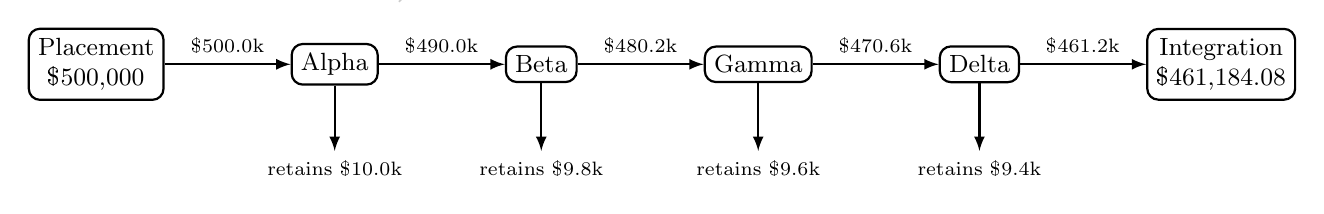
\begin{tikzpicture}[>=latex,thick,node distance=1.6cm]
        \node[draw,rounded corners,align=center,font=\small] (place) {Placement\\\$500{,}000};
        \node[draw,rounded corners,align=center,font=\small,right=of place] (alpha) {Alpha};
        \node[draw,rounded corners,align=center,font=\small,right=of alpha] (beta) {Beta};
        \node[draw,rounded corners,align=center,font=\small,right=of beta] (gamma) {Gamma};
        \node[draw,rounded corners,align=center,font=\small,right=of gamma] (delta) {Delta};
        \node[draw,rounded corners,align=center,font=\small,right=of delta] (integ) {Integration\\\$461{,}184.08};
        \draw[->] (place) -- node[above,font=\scriptsize] {\$500.0k} (alpha);
        \draw[->] (alpha) -- node[above,font=\scriptsize] {\$490.0k} (beta);
        \draw[->] (beta) -- node[above,font=\scriptsize] {\$480.2k} (gamma);
        \draw[->] (gamma) -- node[above,font=\scriptsize] {\$470.6k} (delta);
        \draw[->] (delta) -- node[above,font=\scriptsize] {\$461.2k} (integ);
        \draw[->] (alpha) -- ++(0,-1.1) node[below,font=\scriptsize] {retains \$10.0k};
        \draw[->] (beta) -- ++(0,-1.1) node[below,font=\scriptsize] {retains \$9.8k};
        \draw[->] (gamma) -- ++(0,-1.1) node[below,font=\scriptsize] {retains \$9.6k};
        \draw[->] (delta) -- ++(0,-1.1) node[below,font=\scriptsize] {retains \$9.4k};
    \end{tikzpicture}
\end{lrbox}
\ifdim\wd\bookmeasuredbox<0.65\linewidth
\setlength{\bookcapwidth}{0.65\linewidth}
\else
\setlength{\bookcapwidth}{\wd\bookmeasuredbox}
\fi
\ffigbox[\bookcapwidth]{
\usebox{\bookmeasuredbox}
}{
    \caption{The four-hop layering chain of Table~\ref{tab:layering_network} as a network}
    \label{fig:layering_network}
}
\end{figure}

After four hops, $\$461{,}184.08$, over $92\%$ of the original placed amount, reaches its ultimate destination, with only $\$38{,}815.92$ lost to the network's own retained ``fees'' along the way, having passed through four legally separate entities in under a week. Figure~\ref{fig:layering_network} draws this chain as the network it actually is, rather than as four separate, individually unremarkable rows in a table.

No individual hop in Table~\ref{tab:layering_network} looks obviously wrong; each is a plausible-looking business payment of a plausible size. What is anomalous is the pattern viewed as a network, and each of its three features is a number rather than an impression: a pass-through ratio of exactly $0.98$ at every hop, where a real operating business retains and redeploys most of what it receives; a dwell time under 24 hours, against the weeks a genuine payables cycle takes; and, at every interior node, exactly one party paying in and exactly one party paid out, an in-degree and out-degree of one in the vocabulary of graphs\index{in-degree and out-degree}, where a real supplier has many customers and many suppliers. Each has innocent explanations on its own. All three at once, repeated four hops in a row, do not.

That conjunction is a reason to look, not a conclusion. A factoring company, an escrow agent, or a freight forwarder shows high pass-through and short dwell as a matter of ordinary business, and a sole-source subcontractor genuinely does have one customer and one supplier; what the shape of the network cannot supply on its own is a reason to believe the money is criminal. Three further tests do that work. The first is \emph{commercial substance}\index{commercial substance}: a real intermediary has employees, premises, and counterparties outside this one chain, whereas Alpha has a bank account, an incorporation date shortly before the flows began, and a registered address it shares with dozens of unrelated entities. The second is \emph{common control}: shared directors or beneficial owners, a shared address, telephone number, or device, or four accounts opened at one branch within days of each other, which turns four legally separate companies into one hand moving its own money and has no innocent reading at all. The third is the fee. Two percent of principal, identical at every hop, is a cut rather than a price, because a genuine service is charged for work performed and does not scale exactly with the sum passing through. Only once such corroboration is in hand does an alert amount to the suspicion of criminal origin that a Suspicious Activity Report requires; the graph by itself reports, exactly as Section~\ref{sec:advanced-imbalance} said of any unsupervised flag, that something is unusual rather than that it is a crime.

This is precisely why anti-money-laundering systems increasingly supplement Section~\ref{sec:risk-tiering}'s per-account behavioral scoring with network or graph-based analysis, examining the structure of relationships between accounts rather than any single account's activity alone, since a layering scheme is, by design, constructed so that every individual node in the chain looks unremarkable.

Stated as a learning problem, this is node and subgraph classification on the transaction graph. Community detection isolates tightly connected clusters that ordinary commercial relationships do not produce, and graph neural networks, which Chapter 17 develops on this chapter's own layering network, learn a representation of each account from its neighbors' features as well as its own, so that an account can be scored on the company it keeps rather than only on what it does. The supervision is weak, since confirmed laundering is rare and arrives late, which is why in practice these models rank leads for investigators instead of deciding anything.

Figure~\ref{fig:crime_pipeline} places this rule-based structuring and layering detection alongside the statistical and behavioral tools developed earlier in the chapter, showing how a real institution's monitoring system typically combines several distinct signals before a case ever reaches a human investigator.

\begin{figure}[htbp]
\centering
\begin{lrbox}{\bookmeasuredbox}
    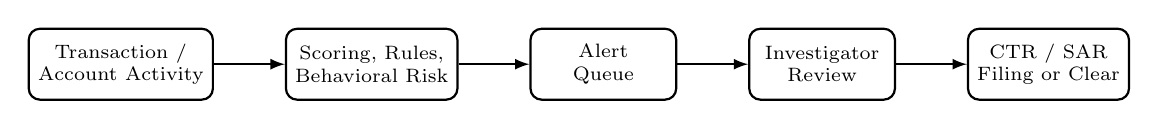
\begin{tikzpicture}[>=latex,thick,node distance=0.9cm]
        \node[draw,rounded corners,minimum width=1.85cm,minimum height=0.9cm,align=center,font=\scriptsize] (txn) {Transaction /\\Account Activity};
        \node[draw,rounded corners,minimum width=1.85cm,minimum height=0.9cm,right=of txn,align=center,font=\scriptsize] (score) {Scoring, Rules,\\Behavioral Risk};
        \node[draw,rounded corners,minimum width=1.85cm,minimum height=0.9cm,right=of score,align=center,font=\scriptsize] (alert) {Alert\\Queue};
        \node[draw,rounded corners,minimum width=1.85cm,minimum height=0.9cm,right=of alert,align=center,font=\scriptsize] (invest) {Investigator\\Review};
        \node[draw,rounded corners,minimum width=1.85cm,minimum height=0.9cm,right=of invest,align=center,font=\scriptsize] (report) {CTR / SAR\\Filing or Clear};
        \draw[->] (txn) -- (score);
        \draw[->] (score) -- (alert);
        \draw[->] (alert) -- (invest);
        \draw[->] (invest) -- (report);
    \end{tikzpicture}
\end{lrbox}
\ifdim\wd\bookmeasuredbox<0.65\linewidth
\setlength{\bookcapwidth}{0.65\linewidth}
\else
\setlength{\bookcapwidth}{\wd\bookmeasuredbox}
\fi
\ffigbox[\bookcapwidth]{
\usebox{\bookmeasuredbox}
}{
    \caption{The fraud and AML monitoring pipeline}
    \label{fig:crime_pipeline}
}
\end{figure}

Beyond structuring, AML regulation imposes an ongoing due-diligence obligation that goes beyond fraud detection's largely reactive posture: Customer Due Diligence (CDD)\index{Customer Due Diligence (CDD)} at onboarding establishes a customer's expected activity profile (Section~\ref{sec:risk-tiering}'s KYC inputs), Enhanced Due Diligence (EDD)\index{Enhanced Due Diligence (EDD)} applies heightened scrutiny to higher-risk customers such as politically exposed persons or those in high-risk jurisdictions, and ongoing monitoring compares actual behavior against that expected profile continuously, the account-level, time-varying risk view Section~\ref{sec:survival-fraud}'s survival framework formalizes.

Two of these obligations are increasingly discharged with the language models Chapter 16 develops. Adverse-media screening, checking whether a customer appears in news reporting tied to fraud, corruption, or sanctions evasion, is a document-classification problem of exactly the kind that chapter's Naive Bayes and embedding methods address, and it inherits this chapter's precision problem in acute form, since most name matches in news text are simply the wrong person. Drafting the suspicious-activity report itself, a structured account of what was observed and why it appears suspicious, is now commonly assisted by a large language model working from the alert's own records. Both uses are governed rather than autonomous: a filed SAR is a legal statement by the institution, so the model proposes and an investigator signs, and the model is itself subject to the validation regime of Section~\ref{sec:governance-3lod}.

\subsection{Sanctions Screening: A Matching Problem, Not a Lookup}\index{Sanctions Screening}
\label{sec:sanctions-screening}

A bank must not move money for a party on a government sanctions list, and unlike almost every other obligation in this chapter, this one admits no risk appetite: the prohibition is absolute, and in the United States liability under the Office of Foreign Assets Control (OFAC)\index{Office of Foreign Assets Control (OFAC)} regime is strict, meaning a bank that processes a prohibited payment has violated the law whether or not it knew, intended, or profited.

It is tempting to conclude from this that sanctions screening is a database lookup rather than a modeling problem. The legal \emph{consequence} of a match is indeed binary, but the \emph{match itself} is not, and conflating the two is the most common way to misunderstand where the difficulty lies. A watchlist records a name in one particular romanization; a payment message arrives carrying whatever spelling, word order, punctuation, and truncation the originating bank's system happened to produce. Nothing guarantees the two strings agree character for character even when they name the same person, and nothing prevents two genuinely different people from having names that differ by a single letter.

The standard tool for comparing two strings that should be the same but are not is the edit distance, or Levenshtein distance\index{Levenshtein distance}, $d(a,b)$: the minimum number of single-character insertions, deletions, or substitutions needed to turn one string into the other, normalized into a similarity score bounded in $[0,1]$,
\begin{equation*}
\text{sim}(a,b) = 1 - \frac{d(a,b)}{\max(|a|,|b|)}.
\end{equation*}
Two short surnames make the mechanics concrete. Turning \texttt{SMITH} into \texttt{SMYTH} requires one substitution, so $d=1$ and $\text{sim} = 1 - 1/5 = 0.800$; turning \texttt{SMITH} into \texttt{SCHMIDT} requires four edits against a longer target, giving $\text{sim} = 1 - 4/7 \approx 0.429$. A screening engine flags any pair scoring above some threshold and sends it to an analyst.

Table~\ref{tab:sanctions_matching} applies this to a watchlist entry, \texttt{Mohammed Al-Rashid}, against seven incoming counterparty names, four of which are the same individual and three of which are not. Scores are computed twice: once after simple normalization (uppercase, punctuation stripped), and once after additionally sorting the name's tokens alphabetically, a standard preprocessing step meant to defeat surname-first ordering.

\begin{table}[htbp]
\centering
\begin{lrbox}{\bookmeasuredbox}
\begin{tabular}{lcrr}
\toprule
Counterparty name & Same person? & Normalized & Token-sorted \\
\midrule
Mohammad Al-Rashid  & yes & 0.9412 & 0.9412 \\
Mohamed Alrashid    & yes & 0.9412 & 0.9412 \\
Muhammad Al-Rasheed & yes & 0.7778 & 0.7778 \\
Al-Rashid, Mohammed & yes & 0.2941 & 1.0000 \\
Mohammed Al-Rashad  & no  & 0.9412 & 0.9412 \\
Ahmed Al-Rashid     & no  & 0.7647 & 0.2941 \\
Mohammed Al-Karim   & no  & 0.7647 & 0.7647 \\
\bottomrule
\end{tabular}
\end{lrbox}
\ifdim\wd\bookmeasuredbox<0.65\linewidth
\setlength{\bookcapwidth}{0.65\linewidth}
\else
\setlength{\bookcapwidth}{\wd\bookmeasuredbox}
\fi
\floatbox[\capbot]{table}[\bookcapwidth]{
\usebox{\bookmeasuredbox}
}{
\caption{Name-similarity scores against the watchlist entry \texttt{Mohammed Al-Rashid}}
\label{tab:sanctions_matching}
}
\end{table}

Token sorting earns its place immediately: \texttt{Al-Rashid, Mohammed} is the same name written surname-first, and plain edit distance scores it $0.2941$, below every non-match in the table, because reversing two words costs almost as many edits as rewriting the string. Sorting the tokens first raises it to a perfect $1.0000$. The same step also pushes \texttt{Ahmed Al-Rashid}, a different person, down from $0.7647$ to $0.2941$, improving separation in both directions at once.

The result that matters, though, is the one no amount of preprocessing fixes. \texttt{Mohammed Al-Rashad}, a different individual whose family name differs from the target's by a single vowel, scores $0.9412$, tying \emph{exactly} with two of the four genuine matches, while the weakest genuine match, \texttt{Muhammad Al-Rasheed}, scores only $0.7778$. The highest-scoring non-match therefore outranks a true match, and no threshold whatsoever separates the two classes: set the bar at $0.90$ and the engine clears a sanctioned party while flagging an innocent one; set it at $0.75$ and it catches everything at the cost of flagging almost everyone.

This is not a defect in the Levenshtein metric that a better string distance would repair. It is a statement about the information content of a name: a name alone does not identify a person, and two of these strings are simply too close for any function of the characters to tell apart. Production screening systems accordingly treat the string score as a first-stage filter and resolve the remainder with secondary identifiers, date of birth, nationality, passport or national identity number, and address, which is precisely why the Know-Your-Customer records collected at onboarding (Section~\ref{sec:risk-tiering}) do double duty as screening inputs rather than sitting inertly in a compliance file.

The strict-liability point now bites. Section~\ref{sec:fraud-scoring}'s threshold choice was an economic trade-off, and Section~\ref{sec:alert-economics} prices it in analyst hours; here one missed true match is a legal violation regardless of how favorable the arithmetic looks, so a bank cannot buy precision by accepting a little less recall. It sets the threshold low enough to make a miss nearly impossible and absorbs whatever false-positive volume results. That inverted operating point is what makes screening expensive.

The scale follows directly. Suppose a mid-sized bank screens $1{,}200{,}000$ payment messages a month against consolidated watchlists, that $15$ of them genuinely involve a sanctioned party, and that a threshold set for near-certain recall produces a $0.5\%$ false-positive rate against the remaining traffic. Then
\begin{equation*}
\text{Alerts} = 0.99(15) + 0.005(1{,}199{,}985) \approx 6{,}015, \qquad \text{Precision} = \frac{14.85}{6{,}015} \approx 0.00247,
\end{equation*}
so roughly $0.25\%$ of screening alerts are genuine, against the $3.0\%$ alert-to-SAR conversion Section~\ref{sec:alert-economics} computed for transaction monitoring: a precision twelve times worse. At $10$ minutes of analyst time per screening alert, half what an AML alert takes because most are cleared on sight, and the same fully loaded \$45 hourly cost,
\begin{equation*}
\text{Analyst hours} = \frac{6{,}015 \times 10}{60} \approx 1{,}002, \qquad \text{Monthly cost} \approx 1{,}002 \times \$45 \approx \$45{,}100,
\end{equation*}
or roughly \$541,000 a year. This is a second alert queue, three-quarters the size of the $8{,}000$-alert transaction-monitoring queue in Section~\ref{sec:alert-economics}, running at one-twelfth its precision, and it exists at every institution that moves money across borders. Supervised learning enters here for a reason worth stating, because labels are abundant in screening where they are scarce almost everywhere else in this chapter: every alert is adjudicated by an analyst, so a bank accumulates hundreds of thousands of match and no-match decisions a year as a by-product of doing the work. A classifier trained on those dispositions scores a candidate pair on far more than string distance, on how common the name is in the relevant population, whether date of birth, nationality, and document number agree, whether the two spellings belong to the same transliteration family, and which kind of list entry was matched; and because it \emph{ranks} rather than thresholds, it can hold recall fixed while pushing most false positives below the line at which the queue is worked. That is the concrete form of the improvement this section has been describing.

Supervised learning enters here for a reason worth stating, because labels are abundant in screening where they are scarce almost everywhere else in this chapter: every alert is adjudicated by an analyst, so a bank accumulates hundreds of thousands of match and no-match decisions a year as a by-product of doing the work. A classifier trained on those dispositions scores a candidate pair on far more than string distance, on how common the name is in the relevant population, whether date of birth, nationality, and document number agree, whether the two spellings belong to the same transliteration family, and which kind of list entry was matched; and because it \emph{ranks} rather than thresholds, it can hold recall fixed while pushing most false positives below the line at which the queue is worked. That is the concrete form of the improvement this section has been describing.

A reader who takes only one operational fact from this chapter should take this one: in most banks, name screening, not transaction monitoring, is the largest single source of compliance alerts, and reducing its false-positive rate without touching recall is among the highest-value applications of machine learning anywhere in financial crime compliance.

\subsection{Privacy-Preserving Collaboration: Federated Learning Across Institutions}
\label{sec:federated-aml}

The layering networks above expose a structural weakness in single-institution detection: a laundering scheme deliberately spreads its transactions across many banks precisely so that no single bank sees enough of the pattern to recognize it. The obvious remedy, pooling transaction data across institutions, is largely prohibited: bank-secrecy and data-protection law restricts sharing customer data, and no bank wants its transaction records in a competitor's hands. Federated learning\index{federated learning} is the machine-learning answer to this impasse: institutions jointly train one shared model \emph{without any of them ever transmitting its underlying data}, by exchanging only model updates. Each bank fits the current shared model to its own private transactions, sends back only the resulting parameter estimates, and a coordinator combines them, most simply by federated averaging\index{federated averaging}, a sample-size-weighted mean of the local estimates, into the next version of the shared model.

A hand-checkable round makes the mechanics concrete. Suppose three banks jointly train the fraud-scoring logistic regression of Section~\ref{sec:fraud-scoring} on a shared structuring-intensity feature, holding $2{,}000$, $5{,}000$, and $3{,}000$ labeled transactions respectively. Their local coefficient estimates come back as $0.90$, $1.30$, and $1.10$: each bank's view is real but partial, and the smallest bank's estimate is the noisiest. Federated averaging weights each estimate by its sample share,
\begin{equation*}
\hat\beta_{\text{fed}} \;=\; \frac{2{,}000 \times 0.90 + 5{,}000 \times 1.30 + 3{,}000 \times 1.10}{10{,}000} \;=\; \frac{11{,}600}{10{,}000} \;=\; 1.16,
\end{equation*}
against a naive unweighted mean of $1.10$; the weighting matters because it lets the estimate lean toward the banks with the most evidence. The payoff is easiest to see from the smallest bank's seat: scoring a transaction with structuring intensity $x=2$ (with intercept $-3$), its own local model flags it with probability $\sigma(-3 + 0.90 \times 2) \approx 0.2315$, while the federated model assigns $\sigma(-3 + 1.16 \times 2) \approx 0.3363$, a meaningfully sharper detector obtained without a single customer record leaving any bank.

Model updates are not automatically harmless, though: a parameter estimate computed from a small dataset can itself leak information about the records behind it, so production systems add differential privacy\index{differential privacy}, calibrated random noise added to each institution's update before transmission, sized so that no observer of the update can reliably infer whether any single transaction was present in the underlying data. The aggregation step is what makes this affordable: perturbing the three local estimates above by illustrative noise draws of $+0.04$, $-0.02$, and $+0.01$ changes the federated coefficient only from $1.16$ to $1.161$, because independent noise largely cancels in a weighted average even while masking each individual contribution. The privacy-utility trade-off does bind, more noise means more privacy and a worse model, and federated systems inherit new operational questions of their own (a malicious participant could poison the shared model through its updates, the adversarial dynamic Chapter 18's robustness discussion examines, transplanted into the training loop), but the core bargain, most of the pooled-data detection gain at none of the pooled-data legal exposure, is why cross-institution federated AML pilots have moved from research into supervised production trials.

\section{Economics and Governance}

A detection model's value is decided by the cost of its false positives and by who is accountable for it. This part is deliberately the shortest in the chapter, and the imbalance is itself the point: detection methods earn their length because they can be taught with worked examples, whereas the failures that actually produce enforcement actions are organizational, and are better shown once and concretely, by the case vignette that follows, than developed at method length.

\subsection{Alert Economics and the Cost of Low Precision}
\label{sec:alert-economics}

Section~\ref{sec:anomaly-bayes} showed that a single bank's fraud model can generate $19{,}600$ flagged transactions in a single day; AML monitoring systems, layering rule-based structuring checks, behavioral risk scores, and sanctions screening on top of transaction scoring, typically generate a comparably large alert volume relative to the number that ultimately warrant a filed report.

Suppose a bank's combined monitoring system generates $8{,}000$ alerts in a typical month, of which $240$ are ultimately investigated and filed as SARs,
\begin{equation*}
\text{Alert-to-SAR conversion rate} = \frac{240}{8{,}000} = 3.0\%,
\end{equation*}
a precision figure of the same qualitative magnitude as Section~\ref{sec:anomaly-bayes}'s $24.2\%$ fraud-flag precision, and considerably lower once every layer of monitoring is combined, since each additional rule or model adds its own false-positive rate. If each alert requires an average of 20 minutes of an investigator's time to review, even the $97\%$ of alerts that are ultimately cleared as false positives,
\begin{equation*}
\text{Analyst hours per month} = \frac{8{,}000 \times 20 \text{ minutes}}{60} \approx 2{,}667 \text{ hours},
\end{equation*}
equivalent to roughly 16 to 17 full-time analysts working a standard month purely to clear the alert queue this single monitoring system generates. At a fully loaded compliance-analyst cost of \$45 per hour, a common industry rule of thumb once salary, benefits, training, and overhead are included, this translates directly into a monthly labor cost of
\begin{equation*}
2{,}666.67 \times \$45 \approx \$120{,}000,
\end{equation*}
or roughly \$1.44 million annually, purely to staff alert review for one monitoring system at one institution, before accounting for the cost of the underlying data infrastructure, the models themselves, or the SAR-filing process that follows a confirmed case. This dollar figure is what makes precision improvements a direct cost-reduction lever rather than merely a statistical nicety.

If a model improvement doubled precision from $3.0\%$ to $6.0\%$ while holding recall (and therefore the $240$ SARs actually filed) fixed, the same $240$ confirmed cases would require only $240/0.06 = 4{,}000$ alerts to surface, exactly half of the original $8{,}000$, cutting analyst hours to $4{,}000 \times 20/60 \approx 1{,}333$ hours and monthly labor cost to $1{,}333 \times \$45 \approx \$60{,}000$, precisely half of the original \$120,000, since cost scales linearly with alert count once recall (and therefore the fixed number of investigations that must occur regardless of precision) is held constant.

This is why a bank's compliance technology budget and its model-development priorities are, in practice, set jointly rather than by the compliance and modeling functions independently: a data-science team's precision improvement translates directly, dollar for dollar, into the compliance department's staffing budget in a way few other model performance metrics do. This is precisely why the layered approach developed in this chapter, transaction scoring (Section~\ref{sec:fraud-scoring}), behavioral risk tiering (Section~\ref{sec:risk-tiering}), and survival-informed prioritization (Section~\ref{sec:survival-fraud}), matters as much for its operational cost efficiency as for its detection accuracy. A monitoring system that better ranks alerts by true risk, even without changing its overall recall, lets a fixed investigative staff spend its limited hours on the alerts most likely to be genuine. That is the same precision-recall trade-off Chapter 6 introduced, now expressed directly in analyst-hours and dollars rather than as an abstract statistical metric.

\subsection{Governance: Model Risk Management and the Three Lines of Defense}
\label{sec:governance-3lod}

Chapters 8 and 9 introduced model risk management\index{model risk management}, independent validation, ongoing performance monitoring, and clear accountability for a model's use, in the context of market and credit risk models; Chapter 14 revisited the same discipline for algorithmic trading systems after the Knight Capital\index{Knight Capital trading glitch} vignette. Fraud and AML models carry an additional governance obligation beyond the purely financial risk those earlier chapters addressed: a poorly governed AML program exposes the institution itself to direct regulatory and criminal liability, not merely financial loss, since failing to detect and report money laundering is, in most jurisdictions, itself a legal violation regardless of whether the institution profited from it.

Banks and regulators structure this accountability using the three lines of defense\index{three lines of defense} framework that Chapter 8's risk-governance section develops in full, and the structure itself carries over unchanged: business units own the first line, an independent compliance and risk function the second, internal audit the third. What differs in the financial-crime setting is what each line is accountable \emph{for}. The second line here builds and validates the scoring and monitoring models this chapter has developed rather than the VaR models of Chapter 8, and the third line's independent testing is itself subject to regulatory examination, so a weak audit function is not merely an internal control gap but a finding a supervisor can act on directly.

This structure is a direct, institutionalized answer to a failure mode this chapter's case vignette illustrates concretely: a monitoring system can exist on paper, and even generate the alert volumes quantified in Section~\ref{sec:alert-economics}, while still failing in practice if the first line lacks the incentive or staffing to act on alerts, if the second line's independent challenge is weak or under-resourced, or if the third line's audits are not, in fact, independent of the business they are reviewing.

\subsubsection*{Model Monitoring: Precision Drift and Adversarial Adaptation}

Chapter 14 introduced concept drift, a predictive model's fitted relationship growing stale as market conditions change, as a reason high-frequency trading models require frequent retraining. Fraud and AML models face a related but distinct version of the same problem: because Section~\ref{sec:crime-taxonomy} identified financial crime as adversarial, fraudsters and launderers who learn (directly or by trial and error) which transaction patterns a bank's model tends to flag will deliberately shift their behavior away from those patterns, degrading the model's precision even if the underlying population of legitimate customers has not changed at all. Table~\ref{tab:precision_drift} illustrates a stylized six-month trajectory for the fraud-scoring model of Section~\ref{sec:fraud-scoring}, holding its classification threshold fixed.

\begin{table}[htbp]
\centering
\begin{lrbox}{\bookmeasuredbox}
\begin{tabular}{lrrrrrr}
\toprule
Month & 1 & 2 & 3 & 4 & 5 & 6 \\
Precision & 24.2\% & 22.5\% & 20.8\% & 19.6\% & 18.3\% & 17.1\% \\
\bottomrule
\end{tabular}
\end{lrbox}
\ifdim\wd\bookmeasuredbox<0.65\linewidth
\setlength{\bookcapwidth}{0.65\linewidth}
\else
\setlength{\bookcapwidth}{\wd\bookmeasuredbox}
\fi
\floatbox[\capbot]{table}[\bookcapwidth]{
\usebox{\bookmeasuredbox}
}{
\caption{An illustrative six-month precision drift at a fixed classification threshold. The trajectory is constructed to show the shape, not measured from a real portfolio.}
\label{tab:precision_drift}
}
\end{table}

If the second line has set a minimum acceptable precision floor of $20\%$ below which the alert-economics burden of Section~\ref{sec:alert-economics} is judged too costly relative to the fraud actually being caught, Table~\ref{tab:precision_drift} crosses that floor between month 3 and month 4, which should trigger a specific, pre-defined governance response, refitting the model on recent data, adding new features that capture the fraudsters' apparent behavioral shift, or tightening the classification threshold, rather than allowing the model to keep running unchanged simply because no single month's decline looks alarming on its own. This is precisely the kind of ongoing performance monitoring Chapter 8's model risk management framework requires, and it is the second line's specific responsibility under the three-lines-of-defense structure above to define the precision floor in advance and act automatically once it is breached, rather than leaving the decision to the first-line staff who are, understandably, focused on clearing today's alert queue rather than questioning whether the underlying model still works.

\section{Case Vignette: The Danske Bank Estonia Case}\index{Danske Bank Estonia Case}\index{Danske Bank Estonia scandal}

Between roughly 2007 and 2015, the Estonian branch of Danske Bank, Denmark's largest bank, processed an estimated 200 billion euros in payments through a portfolio of non-resident customers, many with connections to Russia and other former Soviet states, that was later found to include large volumes of transactions with no plausible legitimate economic purpose. The branch had inherited this non-resident customer portfolio through an earlier acquisition and, rather than winding it down as a high-risk legacy business, continued serving and even expanding it, drawn by the fee income a small branch's outsized transaction volume generated. An internal whistleblower first raised concerns in 2013; an external investigation the bank itself later commissioned found extensive, longstanding failures in customer due diligence, ongoing monitoring, and the bank's own internal escalation of red flags, precisely the first- and second-line failures Section~\ref{sec:governance-3lod}'s three-lines-of-defense framework is designed to prevent. Estonian authorities ultimately required the branch's closure in 2019, and in 2022 Danske Bank pleaded guilty in the United States to fraud charges connected to the case, agreeing to forfeit and pay roughly \$2 billion.

The case is instructive for this chapter specifically because it was not, primarily, a failure of statistical modeling. Rule-based transaction monitoring, of the kind Section~\ref{sec:aml-structuring} describes, was reportedly in place at the branch. But it generated so many alerts, echoing Section~\ref{sec:alert-economics}'s alert-economics discussion, relative to the compliance staff available to review them, that a large fraction went uninvestigated or were cleared without adequate scrutiny. It is also a case study in correspondent banking risk specifically. Much of the flagged activity moved through the branch's relationships with other banks acting as intermediaries for the ultimate, often difficult-to-identify beneficial owners of the funds. That structural feature of international payments makes a single bank's own customer due diligence, however well executed, an incomplete safeguard on its own. The case's lasting regulatory legacy has been a much closer supervisory focus, across the European Union and beyond, on the governance question Section~\ref{sec:governance-3lod} formalizes. The question is not merely whether a monitoring system technically exists. It is whether an institution can demonstrate, to an independent third line and ultimately to a regulator, that alerts are being investigated and reported at a standard consistent with the risk the underlying customer base actually presents.

\section{Challenges in Fraud Detection, Compliance, and Financial Crime}

Several challenges recur across nearly every application in this chapter, and many connect directly to themes developed elsewhere in this book.

\textbf{Extreme class imbalance makes accuracy a misleading metric.} As Section~\ref{sec:anomaly-bayes}'s scaled Bayes' theorem example showed concretely, even a highly accurate-sounding model produces a large number of false positives in absolute terms whenever the event being detected is rare, which is precisely why this chapter, like Chapter 6's imbalanced-classification discussion, insists on precision, recall, and alert-volume economics rather than raw accuracy.

\textbf{The adversary adapts, which most of this book's other models do not have to contend with.} A credit-scoring model's population of borrowers (Chapter 9) is not actively trying to defeat the model; a launderer engaged in structuring (Section~\ref{sec:aml-structuring}) is specifically designing behavior to evade a known detection rule, meaning a fraud or AML model's effectiveness can decay not just through the ordinary concept drift Chapter 14 discussed for order-flow models, but through deliberate, targeted evasion once a detection threshold becomes known or guessable.

\textbf{Data across institutions and jurisdictions is fragmented.} The correspondent-banking structure behind this chapter's case vignette illustrates a recurring practical limit: any single institution's monitoring system, however well built, only observes its own slice of a transaction chain that may span several banks and countries, which is why network-level and cross-institutional information sharing, within the legal limits privacy and banking secrecy law impose, materially improves detection relative to any one institution acting alone, and why the federated learning of Section~\ref{sec:federated-aml} is worth the operational complexity it adds.

\textbf{False positives carry a real customer and reputational cost, not just an operational one.} Every incorrectly frozen account or declined transaction identified in Section~\ref{sec:alert-economics}'s alert queue is also a legitimate customer temporarily denied normal use of their own funds, a cost that does not show up in a precision or recall statistic but matters directly to customer relationships and, in aggregate, to regulatory scrutiny of whether a program's false-positive rate is itself proportionate.

\textbf{Explainability requirements constrain model choice.} As Chapter 18 develops further, a suspicious activity report or an account closure decision frequently must be explained to a regulator or, in some jurisdictions, to the customer, which limits how much a fraud or AML program can rely on the least interpretable models Chapter 6 introduced, in tension with those models' potential accuracy advantage.

\textbf{Governance failures, not modeling failures, are the more common root cause of large-scale enforcement actions.} The Danske Bank Estonia case, like the Knight Capital vignette in Chapter 13, illustrates that the binding constraint is frequently not the sophistication of the detection model but whether the organization around it, staffing, escalation, independent challenge, and audit, actually functions as the three-lines-of-defense framework in Section~\ref{sec:governance-3lod} assumes it does on paper.

\section{Key Takeaways}

Fraud detection and anti-money-laundering compliance apply the classification tools Chapter 6 developed and Chapter 9 specialized to credit risk to a domain defined by extreme class imbalance and an adversary that actively adapts to known detection rules. Beyond a single logistic regression, production systems draw on a broader toolkit developed in Section~\ref{sec:advanced-imbalance}: class weighting and resampling techniques such as SMOTE address the imbalance directly, tree-based ensembles capture nonlinear feature interactions a purely additive model misses, unsupervised anomaly detection catches patterns no confirmed label yet describes, and precision-recall AUC, not ROC-AUC, is the evaluation metric suited to a rare-event problem like this one.

Chapter 1's Bayes' theorem fraud example, scaled to a full day of transaction volume and re-applied to insider trading surveillance, shows concretely why even an apparently accurate model generates a large false-positive alert queue, and that precision at a low base rate is far more sensitive to the false-positive rate than to the true-positive rate, so alert economics, not just statistical accuracy, must guide how a fraud or AML program is designed and staffed.

A single-transaction scoring model, however well fit, structurally cannot catch a fraud that looks unremarkable in isolation, which motivates account-level behavioral risk tiering and, this chapter's methodologically new contribution, survival analysis, the Kaplan-Meier estimator, to characterize how account risk accumulates and resolves over time using both confirmed events and censored observations.

Two growing fraud types defeat transaction-level scoring outright rather than merely straining it. A synthetic identity has no victim to report it, so its losses are booked as ordinary credit loss and never reach a supervised model's training labels at all, which is the strongest case in this chapter for unsupervised detection and for linkage analysis across accounts. An authorized push payment scam is genuinely authorized by the customer, so no feature of the payment itself carries signal, and detection must move to the customer's own baseline and to the beneficiary account; mandatory reimbursement is what turned that from a customer-education problem into an expected-cost calculation a bank can solve.

Sanctions screening looks like a lookup and is in fact a matching problem: Section~\ref{sec:sanctions-screening}'s worked example shows a non-match tying exactly with two genuine matches on name similarity alone, so no threshold separates them and secondary identifiers must finish the job. Because liability for a missed match is strict, recall cannot be traded for precision the way it can everywhere else in this chapter, which is why name screening is typically a bank's largest single alert queue and its least precise one.

Anti-money-laundering regulation adds a reporting and due-diligence apparatus, CTRs, SARs, KYC, and sanctions screening, with no direct counterpart in ordinary credit or fraud risk modeling, built specifically around legally defined thresholds that launderers attempt to evade through the placement-layering-integration sequence, structuring at the placement stage and shell-entity network chains at the layering stage. The Danske Bank Estonia case shows that the binding constraint on a compliance program is at least as often organizational, whether the three lines of defense actually function independently, as it is statistical, and that governance discipline, not just modeling sophistication, is what separates a monitoring system that works on paper from one that works in practice.

\section{Suggested Exercises}

\begin{enumerate}
    \item A different fraud model achieves a 90\% true-positive rate and a 1\% false-positive rate at the same 1\% fraud prevalence Chapter 1 assumed. Using Bayes' theorem, compute the resulting precision, and explain why a lower false-positive rate improved precision more than the higher true-positive rate in Chapter 1's original model.
    \item Using the insider trading surveillance example in Section~\ref{sec:anomaly-bayes}, recompute $\Pr(\text{Insider}\mid\text{Flag})$ if the false-positive rate is reduced from 8\% to 4\%, holding the 2\% base rate and 75\% true-positive rate fixed, and compare the size of this improvement to what a similarly sized improvement in the true-positive rate alone would produce.
    \item Using Table~\ref{tab:fraud_scoring_data}, suppose an eleventh transaction has an amount $z$-score of 2.2, a distance of 4.0 (hundreds of km), and occurs during the day (late-night flag 0). Using the fitted coefficients in Section~\ref{sec:fraud-scoring}, compute the transaction's predicted fraud probability and classification at a 0.5 threshold.
    \item Explain, referencing transaction 9 in Table~\ref{tab:fraud_scoring_data}, why a transaction-level model can have perfect precision and still leave a bank exposed to fraud, and describe how Section~\ref{sec:risk-tiering}'s behavioral risk tiering could catch the case the transaction-level model missed.
    \item Using Section~\ref{sec:advanced-imbalance}'s class-weighting example, explain why raising transaction 9's predicted probability from $33\%$ to $41.7\%$ was not, by itself, enough to fix the false negative at the original $0.5$ threshold, and why the combination of class weighting and a lower threshold reached the same operating point as simply lowering the unweighted model's threshold to $0.30$.
    \item Explain, in a short paragraph, why ROC-AUC can overstate a fraud model's practical usefulness under the kind of extreme class imbalance this chapter has emphasized, and why precision-recall AUC does not share this weakness.
    \item Using Table~\ref{tab:km_table}'s method, compute the Kaplan-Meier survival estimate for a new sample of 8 flagged accounts with observed times (days, $+$ denotes censored) of 4, 6$^+$, 10, 14, 14$^+$, 22, 28$^+$, 33, showing your calculation at each confirmed-fraud event time.
    \item A customer makes four cash deposits of \$9,200 each within five days. Compute the total deposited, and explain, using Section~\ref{sec:aml-structuring}'s structuring discussion, why no individual deposit triggers a Currency Transaction Report even though the total clearly would if deposited at once.
    \item Using Table~\ref{tab:layering_network}'s method, compute a five-hop layering chain starting from \$300,000, with each entity retaining $3\%$ and forwarding the rest, and report the amount reaching the final destination and the total retained across all five hops.
    \item A bank's monitoring system generates $12{,}000$ alerts per month, of which $180$ become filed SARs, and each alert takes an average of 25 minutes to review. Compute the alert-to-SAR conversion rate and the total analyst-hours required per month, and compare both figures to Section~\ref{sec:alert-economics}'s worked example.
    \item Using Section~\ref{sec:governance-3lod}'s three-lines-of-defense framework, identify which line (first, second, or third) each of the following failures most directly represents, and explain why: (a) a branch employee ignores an internal escalation policy for a suspicious customer; (b) an independent audit team reports directly to the same regional manager whose unit it is auditing; (c) the compliance function never independently tests whether the transaction-monitoring model's alert thresholds are still appropriate.
    \item Pick two of the challenges listed in this chapter and describe a concrete scenario, not already used in the text, in which that challenge could cause a fraud or AML program to fail despite a well-designed underlying statistical model, and explain briefly why adding more computing power or a more flexible model would not, by itself, resolve either scenario you describe.
    \item Explain, using the Danske Bank Estonia case vignette, why correspondent banking relationships make financial crime detection harder for any single institution acting alone, and describe one mechanism (discussed in this chapter or otherwise), such as cross-institution information sharing or a shared utility for sanctions and beneficial-ownership screening, that could mitigate this limitation.
    \item Compare the class-imbalance problem in this chapter's fraud examples to the loan-default classification example in Chapter 6: using Chapter 6's confusion matrix (a 75\% true-positive rate and, among the six actual non-defaulters, one false positive), compute what the loan portfolio's default rate would need to be, holding the same true-positive and false-positive rates constant, for precision to fall to the same 24.2\% level as this chapter's fraud example.
    \item Using Greenwood's formula, compute $\widehat{\text{Var}}[\hat S(12)]$ and the resulting 95\% confidence interval for $\hat S(12)\approx0.7407$, and compare its width to the width of the interval already computed at $t=20$ in the text, explaining why the earlier time point's interval is narrower even though both are computed from the same 12 accounts.
    \item Using Section~\ref{sec:sanctions-screening}'s similarity definition, compute $\text{sim}$ for the pairs \texttt{MOHAMMED ALRASHID}/\texttt{MUHAMMED ALRASHID} and \texttt{MOHAMMED ALRASHID}/\texttt{MOHAMMED ALRASHEED}, and explain why the second pair, which involves a genuinely different family name, nonetheless scores higher than \texttt{Muhammad Al-Rasheed} does in Table~\ref{tab:sanctions_matching}.
    \item Using Section~\ref{sec:sanctions-screening}'s screening-volume example, recompute the monthly alert count, precision, analyst hours, and dollar cost if a better matching engine cut the false-positive rate from $0.5\%$ to $0.2\%$ while holding recall at $99\%$, and express the annual saving relative to the \$541,000 figure in the text. Then compute what the same $60\%$ reduction in false positives would save in Section~\ref{sec:alert-economics}'s transaction-monitoring queue, and explain why a bank might nonetheless prioritize the screening engine even though the transaction-monitoring saving turns out to be the larger of the two.
    \item Explain why a bank cannot manage its sanctions-screening alert volume the way Section~\ref{sec:fraud-scoring} manages its fraud-scoring alert volume, by raising the classification threshold, and describe what a screening program can change instead in order to reduce false positives without reducing recall.
    \item Using Section~\ref{sec:new-fraud-types}'s cultivation arithmetic, recompute the bust-out for a synthetic identity that grows \emph{six} tradelines to a \$7,500 limit each over 24 months while paying \$150 a month across all of them. Report the amount paid in, the exposure at bust-out, the net loss, and the return on the fraudster's outlay, and explain why the return multiple is lower here than the text's despite the larger absolute loss.
    \item Suppose the reimbursement rules of Section~\ref{sec:new-fraud-types} were tightened so the sending bank bore $100\%$ of authorized push payment losses rather than half. Holding the $500{,}000$ monthly payments, $0.02\%$ scam rate, \$4,200 average loss, $60\%$ recall, $5\%$ precision, 15-minute intervention and \$45 hourly cost fixed, recompute the loss prevented, the net monthly benefit, and the break-even recall, and comment on what the change in break-even recall implies about how much detection effort a bank would rationally fund under each regime.
    \item \textbf{Challenge (real data).} Download the Kaggle ``Credit Card Fraud Detection'' dataset (Universit\'e Libre de Bruxelles; roughly 285,000 European cardholder transactions over two days, with 492 confirmed frauds and features already anonymized via PCA). Its $0.172\%$ fraud rate is far more extreme than Table~\ref{tab:fraud_scoring_data}'s ten-transaction toy example. (a) Fit a logistic regression with and without class weighting, as in Section~\ref{sec:advanced-imbalance}, and report precision, recall, $F_1$, and precision-recall AUC for both, since accuracy alone is uninformative at this imbalance. (b) Using Section~\ref{sec:alert-economics}'s cost-based framework and assuming a \$50 review cost per flagged transaction and a \$200 average loss per missed fraud, find the threshold that minimizes total expected cost, and compare its alert volume to what a naive $0.5$ threshold would produce. (c) Since the features are already anonymized PCA components rather than raw transaction attributes, this dataset cannot support the same kind of domain-driven feature engineering (for example, distance from home) used in this chapter's own toy example; discuss what information a real bank's fraud team has access to that this public, privacy-scrubbed dataset deliberately withholds.
\end{enumerate}

\section{Further Reading}

\begin{itemize}
    \item Bolton and Hand, ``Statistical Fraud Detection: A Review,'' \emph{Statistical Science}. A foundational survey of statistical approaches to fraud detection, including the class-imbalance and base-rate issues central to Section~\ref{sec:anomaly-bayes}.
    \item Chawla, Bowyer, Hall, and Kegelmeyer, ``SMOTE: Synthetic Minority Over-sampling Technique,'' \emph{Journal of Artificial Intelligence Research}. The original paper introducing the resampling technique discussed in Section~\ref{sec:advanced-imbalance}.
    \item Klein, \emph{Survival Analysis: Techniques for Censored and Truncated Data}. A standard, thorough reference on the Kaplan-Meier estimator and censoring introduced in Section~\ref{sec:survival-fraud}.
    \item Financial Action Task Force (FATF), \emph{International Standards on Combating Money Laundering and the Financing of Terrorism and Proliferation}. The primary international regulatory framework underlying the KYC, CDD, and reporting obligations discussed in Section~\ref{sec:aml-structuring}.
    \item U.S. Department of the Treasury, Office of Foreign Assets Control, \emph{A Framework for OFAC Compliance Commitments}. The regulator's own statement of what a sanctions compliance program must include, and the primary source for the strict-liability standard underlying Section~\ref{sec:sanctions-screening}.
    \item U.S. Financial Crimes Enforcement Network (FinCEN), \emph{Bank Secrecy Act Regulations and Guidance}. The primary U.S. regulatory source for the CTR and SAR reporting requirements discussed in this chapter.
    \item Bruun \& Hjejle, \emph{Report on the Non-Resident Portfolio at Danske Bank's Estonian Branch}. The external investigation commissioned by Danske Bank itself, the primary source for the factual account in this chapter's case vignette.
    \item Institute of Internal Auditors, \emph{The Three Lines Model: An Update of the Three Lines of Defense}. The current authoritative statement of the governance framework developed in Section~\ref{sec:governance-3lod}.
\end{itemize}

\end{document}

